\documentclass{standalone}

\begin{document}

\subsection[CT Dataset]{Femur CT Dataset}\label{segmentation:ct}

The training of a deep Neural Network model as the U-Net requires a large set of images with corresponding labels.
We developed some experiments on automatic segmentation into a (work in progress) project commissioned by the Rizzoli Hospital of Bologna.
The project aims to develop an automatic pipeline of image processing to extract the 3D femur structure starting from CT (\emph{Computer Tomography}) images.
In particular, the crucial point is to improve femur head identification and segmentation, trying to discriminate this part of the bone from the articular cartilage and, moreover, acetabular fossa.
The project was developed in collaboration with the Engineering group of the professor Viceconti and it aims to study the osteoporosis syndrome and its consequences.

In this work no data have been provided by the Rizzoli Hospital and it is hard to find annotated biomedical (public) images on-line, especially about the region of our interest.
We found only few samples of femur CT images (4 patients) and they are certainly not enough for an accurate training of the model.
Thus, we applied a huge data augmentation pre-processing: each image was randomly rotated, shifted and mirrored.
Moreover, we had to face the problem of data annotation which is always a difficult and time expensive task: we did not have accurate medical annotation, so we had to perform them by ourself.

\begin{figure}[htbp]
\centering
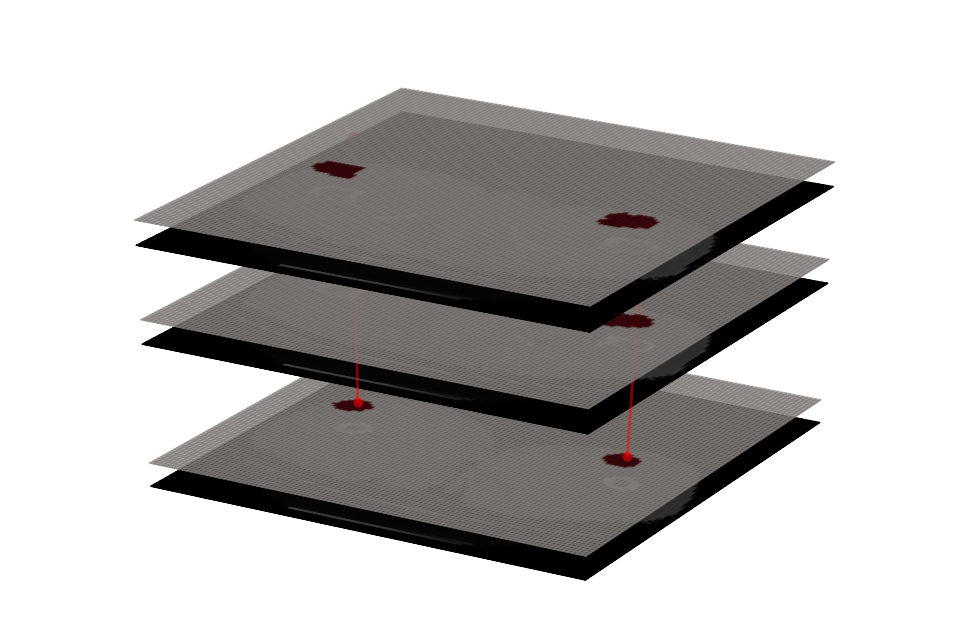
\includegraphics[width=0.85\textwidth]{3D_tool.png}
\caption{Naive segmentation pipeline applied to a series of CT slices.
The thresholding algorithm combined with morphological operations allow to obtained a naive segmentation of the femur bone.
The centroid of the segmented connected components is used to filter the false positive results.
This pipeline was used to simplify the annotation procedure of the CT dataset.
}
\label{fig:3D_tool}
\end{figure}

The annotation was performed using a semi-automatic approach.
We developed a custom image processing pipeline, applying a combination of thresholding and morphological operators to extract as better as possible the bone structure from each CT frame (identified as a pixel connected component).
The thresholding operation produced many false positives into a single image which had to be filtered.
We could (reasonably) assume that the femur position did not change between two following images.
Thus, once the multiple pixel connected components were identified, we filtered them according to their relative position into the image: each group of pixels obtained by thresholding had its own centroid, which it remained quite the same also into the next slice (ref. Fig.\ref{fig:3D_tool}).
An interpolation of these components was performed to filter only the femur parts.
This method worked quite good when we considered slices far from the femur head: when the acetabular fossa became very close to the femur head, the two components were not divided.
An example of this kind of issues is shown in Fig.~\ref{fig:seg_tool}.

\begin{figure}[htbp]
\centering
\def\svgwidth{0.85\textwidth}
\input{./img/segmentation_tool.pdf_tex}
\caption{Example of automatic segmentation using custom image processing pipeline.
Starting from the bottom of femur bone the detection seems good but when the method starts to fail the failure is propagated to the next slices.
The method is too naive to perform a good segmentation on the full set of slices.
However, it can be useful to reduce the quantity of slices to annotate manually.
}
\label{fig:seg_tool}
\end{figure}

This image processing naive approach could not solve the full segmentation task but it can be considered as a good preliminary tool to produce annotated image.
With it we reduced the amount of required annotations by more than 50\%.
The other part of the images were manually annotated.
The manual annotation was performed without any medical background and thus we can not ensure the goodness of our results.
This work only aims to prove the possibility of using deep learning techniques to face segmentation problems.

Following this approach we have been able to annotate $104$ CT images randomly sampled from the $4$ patient slices.
In particular, we have extracted $40$ slices from a single patient and $96$ from the remaining three.
In this way we could use the $96$ images as training set (applying the told above image augmentation) and the $40$ remaining slices as test set.
We chose to use a single patient slices as test set because with the output generated by the U-Net model we want to reconstruct the (approximated) 3D structure of the femur bone.
The 3D reconstruction is still in work in progress and we will not discuss about the obtained results.

\end{document}
